\documentclass{beamer}

\usepackage{url}           % format URLs
\usepackage{listings}      % format code
\lstset{
  mathescape, 
  language={C},
  basicstyle=\small
}
\usepackage{enumitem}      % adjust spacing in enums
%\usepackage[colorlinks=true,allcolors=blue,breaklinks,draft=false]{hyperref}   
\usepackage{graphicx}
\usepackage{float}
\usepackage{subcaption}
\usepackage{xspace,framed}
\usepackage{colortbl}
\usepackage{calc}
%\usepackage[dvipsnames]{xcolor}
\usepackage{amssymb,amsmath,amsfonts} 
\usepackage{mathtools}
\usepackage{microtype}

\usepackage{algorithm}
\usepackage{amsfonts}
\usepackage{multicol}
\usepackage{multirow}
\usepackage{tikz}
\usetikzlibrary{positioning, automata, shapes.arrows, calc, shapes, arrows}
\usetikzlibrary{patterns}
\usepackage[justification=centering]{caption}
\usepackage{stmaryrd}
\usepackage{hhline}
\usepackage{pifont}
\usepackage{pgfplots}
\usepackage{longtable}
\usepackage{afterpage}
\usepackage{wasysym}
\usepackage[scaled]{helvet}
\usepackage{mdwlist}

\newtheorem{myassumption}{Assumption}
\newtheorem{mylemma}{Lemma}
\newtheorem{myprop}{Proposition}

\renewcommand{\baselinestretch}{0.991}
\allowdisplaybreaks
\newcommand\tool{{\sf DSSynth}\xspace}
\newcommand{\xmark}{\ding{55}}


\begin{document}

\title {Sound and Automated Synthesis of Digital Controllers for Continuous Plants}

\author{\textbf{Alessandro Abate}, Iury Bessa, Dario Cattaruzza, Lucas Cordeiro, Cristina David, Pascal Kesseli and Daniel Kroening}

\date{March 2017}

\frame{\maketitle}

\begin{frame}{Cyber-Physical Systems (CPS)}

\begin{itemize}
\item 
modern controls are implemented with digital microcontrollers, 
embedded within dynamical plants representing physical components 
\item 
digital control literature: success and limitations 
\end{itemize} 

\begin{figure}
    \centering
    \begin{subfigure}[b]{0.3\textwidth}
        \includegraphics[width=\textwidth]{figures/step1_figureB.png}
    \end{subfigure}
    ~
    \begin{subfigure}[b]{0.3\textwidth}
        \includegraphics[width=\textwidth]{figures/step1_figureC.png}
    \end{subfigure}
%     ~
%    \begin{subfigure}[b]{0.3\textwidth}
%        \includegraphics[width=\textwidth]{figures/step1_figureD.png}
%    \end{subfigure}
    ~
    \begin{subfigure}[b]{0.3\textwidth}
        \includegraphics[width=\textwidth]{figures/step1_figureA.png}
    \end{subfigure}
\end{figure}

\pause 

\begin{itemize}
\item 
use of counter\-example guided inductive synthesis (CEGIS)\\ 
to automate design of sound digital controllers 
\end{itemize} 

\end{frame}

\begin{frame}[fragile]{CPS Setup: Continuous Plant and Digital Controller}

\begin{figure}[htb]
\centering

\tikzset{add/.style n args={4}{
    minimum width=6mm,
    path picture={
        \draw[circle] 
            (path picture bounding box.south east) -- (path picture bounding box.north west)
            (path picture bounding box.south west) -- (path picture bounding box.north east);
        \node[draw=none] at ($(path picture bounding box.south)+(0,0.13)$)     {\small #1};
        \node[draw=none] at ($(path picture bounding box.west)+(0.13,0)$)      {\small #2};
        \node[draw=none] at ($(path picture bounding box.north)+(0,-0.13)$)    {\small #3};
        \node[draw=none] at ($(path picture bounding box.east)+(-0.13,0)$)     {\small #4};
        }
    }
 }

\resizebox{1.0\textwidth}{!}{
 \begin{tikzpicture}[scale=0.6,-,>=stealth',shorten >=.2pt,auto,
     semithick, initial text=, ampersand replacement=\&,]

  \matrix[nodes={draw, fill=none, shape=rectangle, minimum height=.2cm, minimum width=.2cm, align=center}, row sep=.6cm, column sep=.2cm] {
    \node[draw=none] (r) {$R(z)$};
%   \& \coordinate (aux0);
   \& \node[circle,add={-}{+}{}{}] (circle) {};
   \node[draw=none] (ez) at ([xshift=.9cm,yshift=.2cm]circle)  {$e(z)$};
   \& \node[rectangle,draw,
	minimum width=1cm,
	minimum height=1cm,
        label=\textbf{Controller}] (cz) at ([xshift=.5cm,yshift=0cm]circle) {\sc $\hat{C}(z)$};
   \node[draw=none] (ud) at ([xshift=1cm,yshift=.2cm]cz)  {$U(z)$};
 
 \only<1>{
 \& \node[rectangle,draw,minimum width=3cm,
	minimum height=1.6cm,] (bbdac) {\sc DAC};
 }
 \only<2->{
   \& complexnode/.pic={ 
      \node[rectangle,draw,
	minimum width=4cm,
	minimum height=1.6cm,
	label=\textbf{DAC},] (dac) {};
     \node[circle,add={}{+}{+}{},fill=gray!20] (q2) at ([xshift=-.65cm]dac.center) {};
     \node[draw=none] (q2t)  at ([xshift=-.65cm,yshift=-.65cm]dac.center) {{\sc Q2}};
     \node[draw=none] (v2)  at ([xshift=-.65cm,yshift=1.5cm]dac.center) {$\nu_2(z)$};
     \node[fill=gray!20] (zoh) at ([xshift=.65cm]dac.center) {{\sc ZOH}};} 
     }
   \& \node[rectangle,draw,
	minimum width=1cm,
	minimum height=1cm,
        label=\textbf{Plant}] (gs) {{\sc $\hat{G}(s)$}};
   \node[draw=none] (ud) at ([xshift=-1cm,yshift=.2cm]gs)  {$U(s)$};
   \node[draw=none] (y) at ([xshift=1cm,yshift=.2cm]gs)  {$\hat{Y}(s)$};
 \only<1>{
 \& \node[rectangle,draw,minimum width=4cm,
	minimum height=1.6cm,] (bbadc) {\sc ADC};
 }   
 \only<2->{
   \& complexnode/.pic={ 
     \node[rectangle,draw,
	minimum width=4cm,
	minimum height=1.6cm,
	label=\textbf{ADC},] (adc) {};
   \draw[] ([xshift=-1cm]adc.center) -- ++(0.5,0.2cm);
   \coordinate (switch1) at ([xshift=-1cm]adc.center);
   \coordinate (switch2) at ([xshift=-0.4cm]adc.center);
   \node[circle,add={}{+}{+}{},fill=gray!20] (q1) at ([xshift=1cm]adc.center) {};} 
     \node[draw=none] (q2t)  at ([xshift=1cm,yshift=-.65cm]adc.center) {{\sc Q1}};
   \node[draw=none] (v1)  at ([xshift=1cm,yshift=1.5cm]adc.center) {$\nu_1(z)$};
   }
   \& \coordinate (aux1);
   \& \node[draw=none] (yz) {$\hat {Y}(z)$};\\
   \& \coordinate (aux3);
   \&
   \&
   \& 
   \& 
   \& \coordinate (aux2);\\
  };


  \path[->] (r) edge (circle.west);
  \path[->] (aux1) edge (yz);
  \path (circle.east) edge (cz);
  \only<1> {
   \path
     (cz.east) edge (bbdac.west)
     (bbdac.east) edge (gs.west);
   \path
      (gs.east) edge (bbadc.west)
      (bbadc.east) edge (aux1.west);
  }
   \only<2->{
  \path[->] (v2) edge (q2.north);
  \path  
   (cz.east) edge (q2.west)
   (q2.east) edge (zoh.west)
   (zoh.east) edge (gs.west);
  \path[->] (v1) edge (q1.north);
  \path
   (gs.east) edge (switch1.west)
   (switch2) edge (q1.west)
   (q1.east) edge (aux1.west);
  }
  \path
   (aux1.south) edge (aux2.north)
   (aux2.west) edge (aux3.east); 
  \path[->]  (aux3.north) edge (circle.south);
 \end{tikzpicture}
}
% \caption{Closed-loop digital control system \label{fig:sampledsystem}}
\end{figure}

%\end{frame}

%\begin{frame}[fragile]{Discrete Time Model}

\uncover<3->
{
\begin{figure}[ht]
\centering
\tikzset{add/.style n args={4}{
    minimum width=6mm,
    path picture={
        \draw[circle] 
            (path picture bounding box.south east) -- (path picture bounding box.north west)
            (path picture bounding box.south west) -- (path picture bounding box.north east);
        \node[draw=none] at ($(path picture bounding box.south)+(0,0.13)$)     {\small #1};
        \node[draw=none] at ($(path picture bounding box.west)+(0.13,0)$)      {\small #2};
        \node[draw=none] at ($(path picture bounding box.north)+(0,-0.13)$)    {\small #3};
        \node[draw=none] at ($(path picture bounding box.east)+(-0.13,0)$)     {\small #4};
        }
    }
 }

\resizebox{1.0\textwidth}{!}{
 \begin{tikzpicture}[scale=0.3,-,>=stealth',shorten >=.2pt,auto,
     semithick, initial text=, ampersand replacement=\&,]

  \matrix[nodes={draw, fill=none, shape=rectangle, minimum height=.2cm, minimum width=.2cm, align=center}, row sep=.6cm, column sep=.3cm] {
    \node[draw=none] (r) {$R(z)$};
%   \& \coordinate (aux0);
   \& \node[circle,add={-}{+}{}{}] (circle) {};
   \node[draw=none] (ez) at ([xshift=1cm,yshift=.15cm]circle)  {$e(z)$};
   \& \node[rectangle,draw,
	minimum width=1cm,
	minimum height=1cm,
        label=\textbf{Controller}] (cz) {\sc $\hat{C}(z)$};
   \node[draw=none] (ud) at ([xshift=1cm,yshift=.15cm]cz)  {$U(z)$};
   \& \node[circle,add={}{+}{+}{}] (circle2) {};
   \node[draw=none] (nu2) at ([yshift=1cm]circle2)  {$\nu_2(z)$};
   \& \node[rectangle,draw,
	minimum width=1cm,
	minimum height=1cm,
        label=\textbf{Plant}] (gs) {{\sc $\hat{G}(z)$}};

   \& \node[circle,add={}{+}{+}{}] (circle3) {};
   \node[draw=none] (nu1) at ([yshift=1cm]circle3)  {$\nu_1(z)$};
   \& \coordinate (aux1);
   \& \node[draw=none] (yz) {$\hat Y(z)$};\\
   \& \coordinate (aux3); 
   \&
   \& 
   \& 
   \&
   \& \coordinate (aux2);\\
  };

  \path[->] (r) edge (circle.west);
  \path[->] (nu2) edge (circle2.north);
  \path[->] (nu1) edge (circle3.north);
  \path[->] (aux1) edge (yz);
  \path  
   (circle.east) edge (cz)
   (cz.east) edge (circle2.west)
   (circle2.east) edge (gs.west)
   (gs.east) edge (circle3.west)
   (circle3.east) edge (aux1.west)
   (aux1.south) edge (aux2.north)
   (aux2.west) edge (aux3.east); 
  \path[->]  (aux3.north) edge (circle.south);
 \end{tikzpicture}
}
%\caption{Fully digital equivalent to system in Figure~\ref{fig:sampledsystem} 
%\label{fig:digsystem1}}
\end{figure}
}

\only<4>{
\begin{displaymath}
\hat{G}(z) = (1-z^{-1})\mathcal{Z}\left\lbrace{\mathcal{L}^{-1}\left\lbrace{\frac{\hat{G}(s)}{s}}\right\rbrace_{t=kT}}\right\rbrace
\end{displaymath}
}

%\only<2-3>{
%\begin{displaymath}
%\hat{Y}(z)=\nu_{1}(z)+\hat{G}(z)\tilde{C}(z)R(z)+\hat{G}(z)\nu_{2}(z)-\hat{G}(z)\tilde{C}(z)\hat{Y}(z)
%\end{displaymath}
%}

\only<5>{
\begin{equation*}
\hat{Y}(z) = 
\frac{\hat{G}(z) \tilde{C}(z)}{1+\hat{G}(z) \tilde{C}(z)}R(z) + 
\frac{1}{1+\hat{G}(z) \tilde{C}(z)} \nu_{1}(z) + 
\frac{\hat{G}(z)}{1+\hat{G}(z) \tilde{C}(z)} \nu_{2}(z) 
\end{equation*}
}

\uncover<6>{
Common denominator:
$$\hat{G}_n(z) \tilde{C}_n(z)+\hat{G}_d(z) \tilde{C}_d(z)$$ 
\textcolor{red}{clarify use of tilde C and of hat C }
}

\end{frame}

\begin{frame}{Stability Analysis via Jury's Criterion}

\begin{equation*}
S(z) = \hat{G}_n(z) \tilde{C}_n(z)+\hat{G}_d(z) \tilde{C}_d(z) = \sum_{i=0}^{N_S} c_iz^{N_s-i}, c_0 \neq 0 
\end{equation*}

$$
M=\left( 
\begin{array}{ccc}
v^{(0)}_{1} &\cdots & v^{(0)}_{N_S}\\
v^{(1)}_{1} &\cdots&  v^{(1)}_{N_S}\\
\vdots&\vdots&\vdots\\
v^{(N_S-1)}_{1} &\cdots&  v^{(N_S-1)}_{N_S}\\
\end{array}
\right), $$
%
$$
v_{j}^{(k)}=\left\{
\begin{array}{ll}
c_{j-1}, & k=0\\
0,&k>0 \wedge \mbox{if}~j>N_S-k\\
v_{1}^{(k-1)}-v_{N_S-j}^{(k-1)} . \frac{v_{1}^{(k-1)}}{v_{N_S-k}^{(k-1)}}, &k>0 \wedge  \mbox{if}~j\leq N_S-k\\
\end{array}
\right.
$$
%
$S(z)$ is stable $\Leftrightarrow$
$$
%\phi_\mathit{stability} \equiv 
\textcolor{blue}{S(1) > 0}\ \uncover<2->{\wedge\ \textcolor{blue}{(-1)^{N_S} S(-1) > 0}}\ \uncover<3->{\wedge\ \textcolor{blue}{|c_0| < c_{N_S}}}\ \uncover<4>{\wedge\ \textcolor{blue}{\forall k, v_1^{(k)} > 0}}
$$

\end{frame}

\begin{frame}{Transfer Functions and Uncertainty}

\begin{align*}
\small
\hat{C}(z)&=\frac{\hat{C}_n(z)}{\hat{C}_d(z)}=\frac{\sum_{i=0}^{M_C}(\beta_{i}+\Delta\beta_{i}) z^{-i}}{\sum_{i=0}^{N_C}(\alpha_{i}+\Delta \alpha_{i}) z^{-i}}, \\
\\%\label{plant_tf}
\hat{G}(z)&=\frac{\hat{G}_n(z)}{\hat{G}_d(z)}=\frac{\sum_{i=0}^{M_G}(b_{i}+\Delta b_i) z^{-i}}{\sum_{i=0}^{N_G}(a_{i}+\Delta a_{i}) z^{-i}}.
\end{align*}
%
\begin{itemize}
\item 
$\vec{\beta}$ and $\vec{\alpha}$ -- vectors containing controller coefficients 
\item 
$\vec{b}$ and $\vec{a}$ -- plant coefficients 
\end{itemize}

\end{frame}

\begin{frame}{Sources of Uncertainty}
\setbeamertemplate{itemize items}[square]

\begin{itemize}
\item<1->[1.] Model Parametric Errors (affect $\Delta G(z)$)
\item<2->[2.] Quantisation errors in the ADC, DAC, and controller arithmetics  
(modelled as external noise, do not affect transfer functions)
\item<3->[3.] Roundoff errors in verification process (affect $\Delta S(z)$)
\item<4->[4.] Discretisation errors (affect $\Delta G(z)$ and $\Delta C(z)$) 
\end{itemize}
\end{frame}

\begin{frame}[fragile]{Pole Placement}

\pgfplotsset{grid style={dotted,gray}}
\pgfplotsset{minor grid style={dotted,gray}}
\pgfplotsset{major grid style={dotted,gray}}

\begin{figure}
\centering
\begin{tikzpicture}[scale=1]
\begin{axis}[xmin=-2.5,xmax=2.5,ymin=-2,ymax=2]
\draw[dashed,color=red] (axis cs:0cm,0cm) circle[radius=100];
\node at (axis cs:.7,-.7) [pin={-10:{stable region}},inner sep=0pt] {};
\draw[color=blue] (axis cs:0.5,0.7) ellipse[x radius=5, y radius=15];
\node at (axis cs:.5,.7) [pin={+10:poles},inner sep=0pt] {};
\end{axis}
\end{tikzpicture}
\end{figure}
\end{frame}


%\begin{frame}[fragile]
%\begin{figure}
%\centering
%\begin{tikzpicture}[scale=1]
%\begin{axis}[xmin=-2.5,xmax=2.5,ymin=-2,ymax=2, minor xtick={-2,-1.75, ..., 2}, minor ytick={-2,-1.75, ..., 2}, grid=both]
%\draw[dashed,color=red] (axis cs:0cm,0cm) circle[radius=100];
%\node at (axis cs:.7,-.7) [pin={-10:stable},inner sep=0pt] {};
%\only<1>{
%\draw[color=blue] (axis cs:0.5,0.7)  ellipse[x radius=5, y radius=15];
%\node at (axis cs:.5,.7) [pin={+10:poles},inner sep=0pt] {};
%}
%\only<2>{
%\draw[color=orange] (axis cs:0.5,0.75) ellipse[x radius=5, y radius=15];
%\node at (axis cs:.5,.75) [pin={+10:poles},inner sep=0pt] {};
%}
%\end{axis}
%\end{tikzpicture}
%\end{figure}
%\end{frame}

\begin{frame}[fragile]{Pole Placement}
\begin{figure}
\centering
\begin{tikzpicture}[scale=1]
\begin{axis}[xmin=0,xmax=1.5,ymin=0,ymax=1]
\draw[dashed,color=red] (axis cs:0cm,0cm) circle[radius=100];
\node at (axis cs:.7,-.7) [pin={-10:stable},inner sep=0pt] {};
\draw[color=blue] (axis cs:0.5,0.7) ellipse[x radius=5, y radius=15];
\node at (axis cs:.5,.7) [pin={+10:poles},inner sep=0pt] {};
\end{axis}
\end{tikzpicture}
\end{figure}
\end{frame}

\begin{frame}[fragile]{Pole Placement in a Discretized Domain}

\pgfplotsset{grid style={dotted,gray}}
\pgfplotsset{minor grid style={dotted,gray}}
\pgfplotsset{major grid style={dotted,gray}}

\begin{figure}
\centering
\begin{tikzpicture}[scale=1]
\begin{axis}[xmin=0,xmax=1.25,ymin=0,ymax=1, xtick={0,0.25, ..., 1.25}, ytick={0,0.25, ..., 1.25}, grid=both]
\draw[dashed,color=red] (axis cs:0cm,0cm) circle[radius=100];
\node at (axis cs:.7,-.7) [pin={-10:stable},inner sep=0pt] {};
\only<1>{
\draw[color=blue] (axis cs:0.5,0.7)  ellipse[x radius=5, y radius=15];
\node at (axis cs:.5,.7) [pin={+10:poles},inner sep=0pt] {};
}
\only<2>{
\draw[color=orange] (axis cs:0.5,0.75) ellipse[x radius=5, y radius=15];
\node at (axis cs:.5,.75) [pin={+10:poles},inner sep=0pt] {};
}
\end{axis}
\end{tikzpicture}
\end{figure}
\end{frame}

%
\begin{frame}{Our Objective}

We seek to synthesise a controller where $\Delta \vec{\beta}=0$ and $\Delta \vec{\alpha}=0$ and which stabilizes all plants within a given range of $\Delta \vec{b}$ and $\Delta \vec{a}$. 



\end{frame}

\begin{frame}[fragile]{CEGIS Architecture}
\begin{figure}[htb]
\centering
\resizebox{1.0\textwidth}{!}
{
 \begin{tikzpicture}[scale=0.3,->,>=stealth',shorten >=.2pt,auto, semithick, initial text=, ampersand replacement=\&,]
  \matrix[nodes={draw, fill=none, shape=rectangle, minimum height=.2cm, minimum width=.2cm, align=center
},
          row sep=1cm, column sep=2cm] {
   \coordinate (aux1);
   \& \coordinate (aux2);
   \&;\\
   \node[minimum width=2.5cm, minimum height=0.6cm, fill=gray!20] (synth) {{\sc Synthesize}};
   \&
   complexnode/.pic={ 
     \node[rectangle,draw,dotted,
	minimum width=7cm,
	minimum height=1cm,
        pattern=north west lines, pattern color=gray!20,
	label={\sc Verify},] (verif) {};
     \node[minimum width=2.5cm, minimum height=0.6cm, fill=gray!20] (verif1) at ([xshift=-2cm]verif.center) {{\sc Uncertainty}};
     \node[minimum width=2.5cm, minimum height=0.6cm, fill=gray!20] (verif2) at ([xshift=2cm]verif.center) {{\sc Precision}};
   } 
   \only<1,22>{\& \node[ellipse, fill=gray!20] (done) {{\sc Done}};}\\
   \& \\
   \node[minimum height=0.5cm] (gp) {\sf Closed-loop System Search\\ \only<2-15>{$\textcolor{blue}{FP=\mathbb{R}\langle16,24\rangle}$}\only<16->{$\textcolor{blue}{FP=\mathbb{R}\langle20,28\rangle}$}};
   \&
   complexnode/.pic={ 
     \coordinate (aux);
   \node[minimum height=0.5cm] (bmc) at ([xshift=-2cm]aux.center) {\sf BMC-based\\Verifier};
   \node[minimum height=0.5cm] (fp)  at ([xshift=2cm]aux.center) {\sf Interval Arithmetic\\Verifier};
   }   
    \\
  };

   \only<1,22>{\path (verif2) edge node {} (done);}
   \only<1>{\path ([xshift=5em]synth.south) edge node[align=center] {Inputs} ([xshift=5em]gp.north);}
   \only<2-7,16-17>{\path ([xshift=5em]synth.south) edge node[align=center] {$\textcolor{blue}{\frac{0.0264}{z-0.9998}}$} ([xshift=5em]gp.north);}
   \only<1-2,8,16,18>{\path ([xshift=-5em]gp.north) edge node[align=center] {UNSAT/\\candidate} ([xshift=-5em]synth.south);}
   \only<3-7,17>{\path ([xshift=-5em]gp.north) edge node[align=center] {$\textcolor{blue}{\frac{0z^2+0z+0}{0z^2+0z+0}}$} ([xshift=-5em]synth.south);}
   \only<1-3,8-9,16,18>{\path ([yshift=2em]synth.east) edge node[xshift=-0.5em] {Candidate solution} ([yshift=2em]verif1.west);}
   \only<4-7,17>{\path ([yshift=2em]synth.east) edge node[xshift=-0.5em] {$\textcolor{blue}{\frac{0z^2+0z+0}{0z^2+0z+0}}$} ([yshift=2em]verif1.west);}
   \only<1-4,8-10,16,18-19>{\path  ([xshift=5em]verif1.south) edge node[align=center] {Candidate\\ $P$} ([xshift=5em]bmc.north);}
   \only<5-7,17>{\path  ([xshift=5em]verif1.south) edge node[align=center] {$\textcolor{blue}{\frac{0z^2+0z+0}{0z^2+0z+0}}$} ([xshift=5em]bmc.north);}
   \only<1-5,8-11,16,18-19>{\path  ([xshift=-5em]bmc.north) edge node[align=center]  {UNSAT/\\model} ([xshift=-5em]verif1.south);}
   \only<6-7>{\path  ([xshift=-5em]bmc.north) edge node[align=center]  {$\textcolor{blue}{\frac{0.026506}{1.000610z+1.002838}}$} ([xshift=-5em]verif1.south);}
   \only<1-6,8-12,16,18>{\path ([yshift=-2em]verif1.west) edge node {Counterexample} ([yshift=-2em]synth.east);}
   \only<7>{\path ([yshift=-2em]verif1.west) edge node {$\textcolor{blue}{\frac{0.026506}{1.000610z+1.002838}}$} ([yshift=-2em]synth.east);}
   \only<8-15>{\path ([xshift=5em]synth.south) edge node[align=center] {$\textcolor{blue}{\frac{0.0264}{z-0.9998}}$\\$\textcolor{blue}{\frac{0.026506}{1.000610z+1.002838}}$} ([xshift=5em]gp.north);}
   \only<9-15,19->{\path ([xshift=-5em]gp.north) edge node[align=center] {$\textcolor{blue}{\tilde C(z)}$} ([xshift=-5em]synth.south);}
   \only<10-15>{\path ([yshift=2em]synth.east) edge node[xshift=-0.5em] {$\textcolor{blue}{\frac{12.402664z^2{-}11.439667z{+}0.596756}{4.003906z^2{-}0.287949z{+}0.015625}}$} ([yshift=2em]verif1.west);}
   \only<11-15,20->{\path  ([xshift=5em]verif1.south) edge node[align=center] {$\textcolor{blue}{\tilde C(z)}$} ([xshift=5em]bmc.north);}
   \only<12-15,20->{\path  ([xshift=-5em]bmc.north) edge node[align=center]  {\textcolor{blue}{UNSAT}\\\textcolor{blue}{Pass}} ([xshift=-5em]verif1.south);}
   \only<1-12,16-20>{\path ([xshift=5em]verif2.south) edge node[align=center] {Candidate\\ $P$} ([xshift=5em]fp.north);}
   \only<13-15,21->{\path ([xshift=5em]verif2.south) edge node[align=center] {$\textcolor{blue}{\tilde C(z)}$} ([xshift=5em]fp.north);}
   \only<1-13,16-20>{\path  ([xshift=-5em]fp.north) edge node[align=center]  {True/\\False} ([xshift=-5em]verif2.south);}
   \only<14-15>{\path  ([xshift=-5em]fp.north) edge node[align=center]  {\textcolor{blue}{False}} ([xshift=-5em]verif2.south);}
   \only<15>{\path ([yshift=-2em]verif1.west) edge node {\textcolor{blue}{precision}} ([yshift=-2em]synth.east);}
   \only<17>{\path  ([xshift=-5em]bmc.north) edge node[align=center]  {$\textcolor{blue}{\frac{0.026314}{0.999024z{-}1.004785}}$} ([xshift=-5em]verif1.south);}
   \only<17>{\path ([yshift=-2em]verif1.west) edge node {$\textcolor{blue}{\frac{0.026314}{0.999024z{-}1.004785}}$} ([yshift=-2em]synth.east);}
   \only<18->{\path ([xshift=5em]synth.south) edge node[align=center] {$\textcolor{blue}{\frac{0.0264}{z-0.9998}}$\\$\textcolor{blue}{\frac{0.026314}{0.999024z{-}1.004785}}$} ([xshift=5em]gp.north);}
   \only<19->{\path ([yshift=2em]synth.east) edge node[xshift=-0.5em] {$\textcolor{blue}{\frac{11.035202z^2{+}5.846100z{+}4.901855}{1.097901z^2{+}0.063110z{+}0.128357}}$} ([yshift=2em]verif1.west);}
   \only<21->{\path  ([xshift=-5em]fp.north) edge node[align=center]  {\textcolor{blue}{True}} ([xshift=-5em]verif2.south);}




   \path (aux1) edge (synth.north);
   \path[-]
   (verif2.north) edge node[align=center] {} ([xshift=6.7cm]aux2)
   ([xshift=6.7cm]aux2) edge node[align=center] {Increase Precision} (aux1);

 \end{tikzpicture}
}
\end{figure}
\end{frame}

%\begin{frame}
%
%\begin{itemize*}
%
%\item We automatically generate {\em correct-by-construction} digital
%  controllers using an inductive synthesis approach.  Our application of program
%  synthesis is non-trivial and addresses challenges specific to control
%  systems, such as quantizers and FWL.  In particular, we
%  have found that a two-stage verification engine that continuously refines
%  the precision of the fixed-point representation of the plant yields a
%  speed-up of two orders of magnitude over a conventional one-stage
%  verification engine.
%
%\item Experimental results show that \tool is able to efficiently synthesize
%  stable controllers for a set of intricate benchmarks taken from the
%  literature: the median runtime for our benchmark set considering the
%  faster engine is $48$\,s, i.e., half of the controllers can be synthesized
%  in less than one minute.
%
%\end{itemize*}
%\end{frame}

%
%
%%%%%%%%%%%%%%%%%%%%%%%%%%%%%%%%%%%%%%%%%%%%%%%%%%%%%%%%%%%%%%%%%%%%%%%%%%%%%%%%%%%%%%%
%\subsection{Illustrative Example} \label{sec:running-ex}
%
%We illustrate our approach with a classical cruise control example from the
%literature~\cite{Astrom08}.  It highlights the challenges that
%arise when using finite-precision arithmetic in digital control.  We are
%given a discrete plant model (with a time step of $0.2$\,s), 
%represented by the following $z$-expression:
%%
%\begin{equation}
%\label{Eq:running-example-plant}
%G(z) = \frac{0.0264}{z-0.9998}.
%\end{equation}
%
%Using an optimization tool, the authors
%of~\cite{DBLP:conf/hybrid/WangGRJF16} have designed a high-performance
%controller for this plant, which is characterized by the following
%$z$-domain transfer function:
%%
%\begin{equation}
%\label{Eq:running-example-controller}
%C(z) = \frac{2.72z^2 - 4.153z + 1.896}{z^2 - 1.844z + 0.8496}.
%\end{equation}
%%
%The authors of~\cite{DBLP:conf/hybrid/WangGRJF16} claim that the controller
%$C(z)$ in~\eqref{Eq:running-example-controller} stabilizes the closed-loop
%system for the discrete plant model $G(z)$
%in~\eqref{Eq:running-example-plant}.  However, if the effects of
%finite-precision arithmetic are considered, then this closed-loop system
%becomes unstable.
%%
%For instance, an implementation of $C(z)$ using 
%$\mathbb R \param {4}{16}$ fixed-point
%numbers (i.e., $4$ bits for the integer part and $16$ bits for the
%fractional part) can be modeled as: 
%%
%\begin{equation}
%\label{Eq:running-example-controller-quantized}
%\resizebox{.47\textwidth}{!}{
%$\tilde{C}(z) {:=} \frac{2.7199859619140625z^2{-}4.1529998779296875z
%{+}1.89599609375}{z^2{-}1.843994140625z+0.8495941162109375}$. 
%}
%\end{equation} 
%%
%The resulting system, 
%%using the typical series loop configuration, 
%where $\tilde{C}(z)$ and $G(z)$ are in the forward path, is unstable. 
%Notice that this is disregarding further approximation effects on the plant caused by quantization in the verifier (i.e., $\tilde{G}(z)$).
%%\aabatecmt{[hang in there - did we not consider FWL on $G(z)$? why not?]}
%%\dariocmt{we are explaining the case where a real plant (no FWL) is not correctly stabilized by $\tilde{C}$, so although our analysis might evaluate $\tilde{G}(z)$, the problem statement is over $G(z)$}
%Figure~\ref{fig:original} gives the Bode diagram for the digital controller
%represented in~\eqref{Eq:running-example-controller}: 
%as the phase margin is negative, 
%the controller is unstable when considering the FWL effects.
%
%
\begin{frame}[fragile]{Step Response for the Candidate Solutions}
\begin{figure}
    \centering
    \begin{subfigure}[b]{0.3\textwidth}
        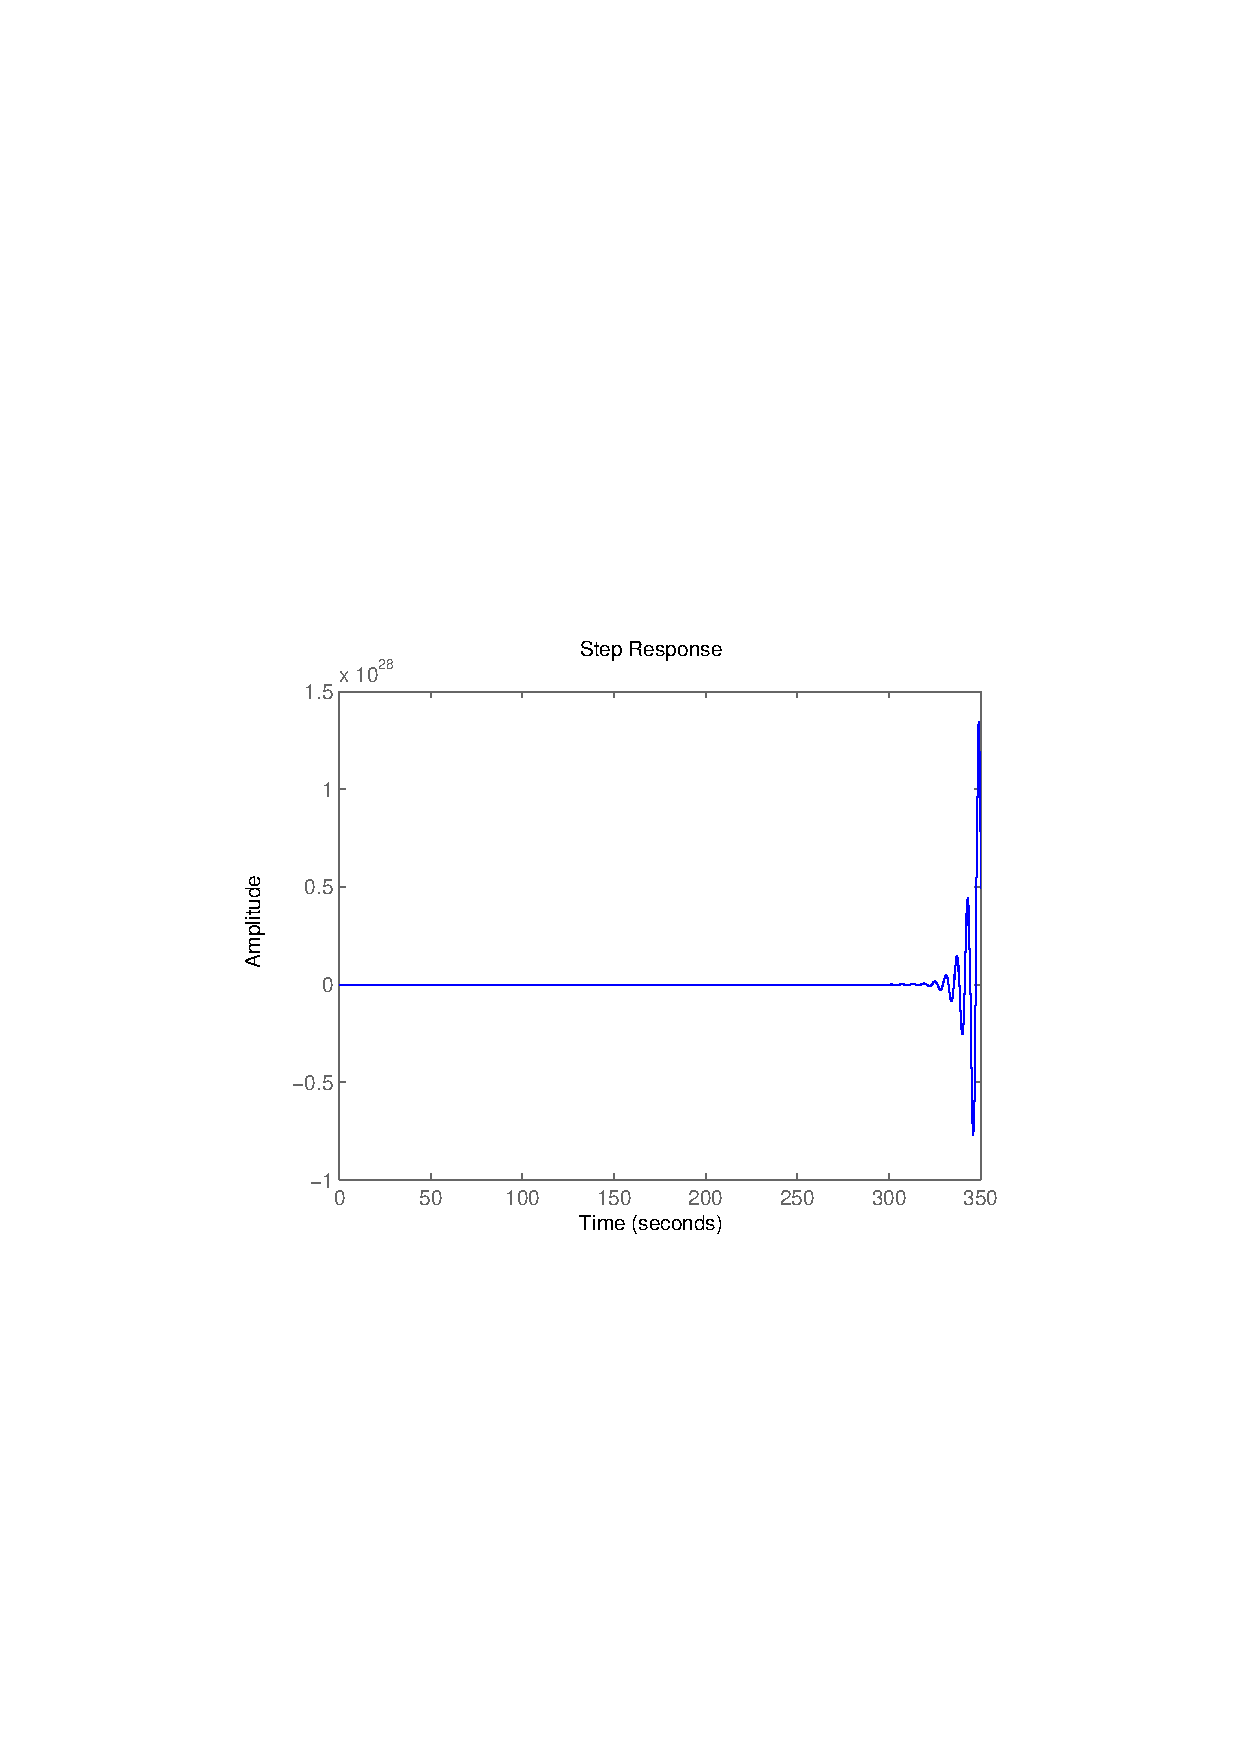
\includegraphics[width=\textwidth]{figures/runningexample_step0.pdf}
        \caption{Original controller}
        \label{fig:step0}
    \end{subfigure}
    ~
    \begin{subfigure}[b]{0.3\textwidth}
        \includegraphics[width=\textwidth]{figures/runningexample_step1.pdf}
        \caption{First solution by \tool}
        \label{fig:step1}
    \end{subfigure}
    ~
    \begin{subfigure}[b]{0.3\textwidth}
        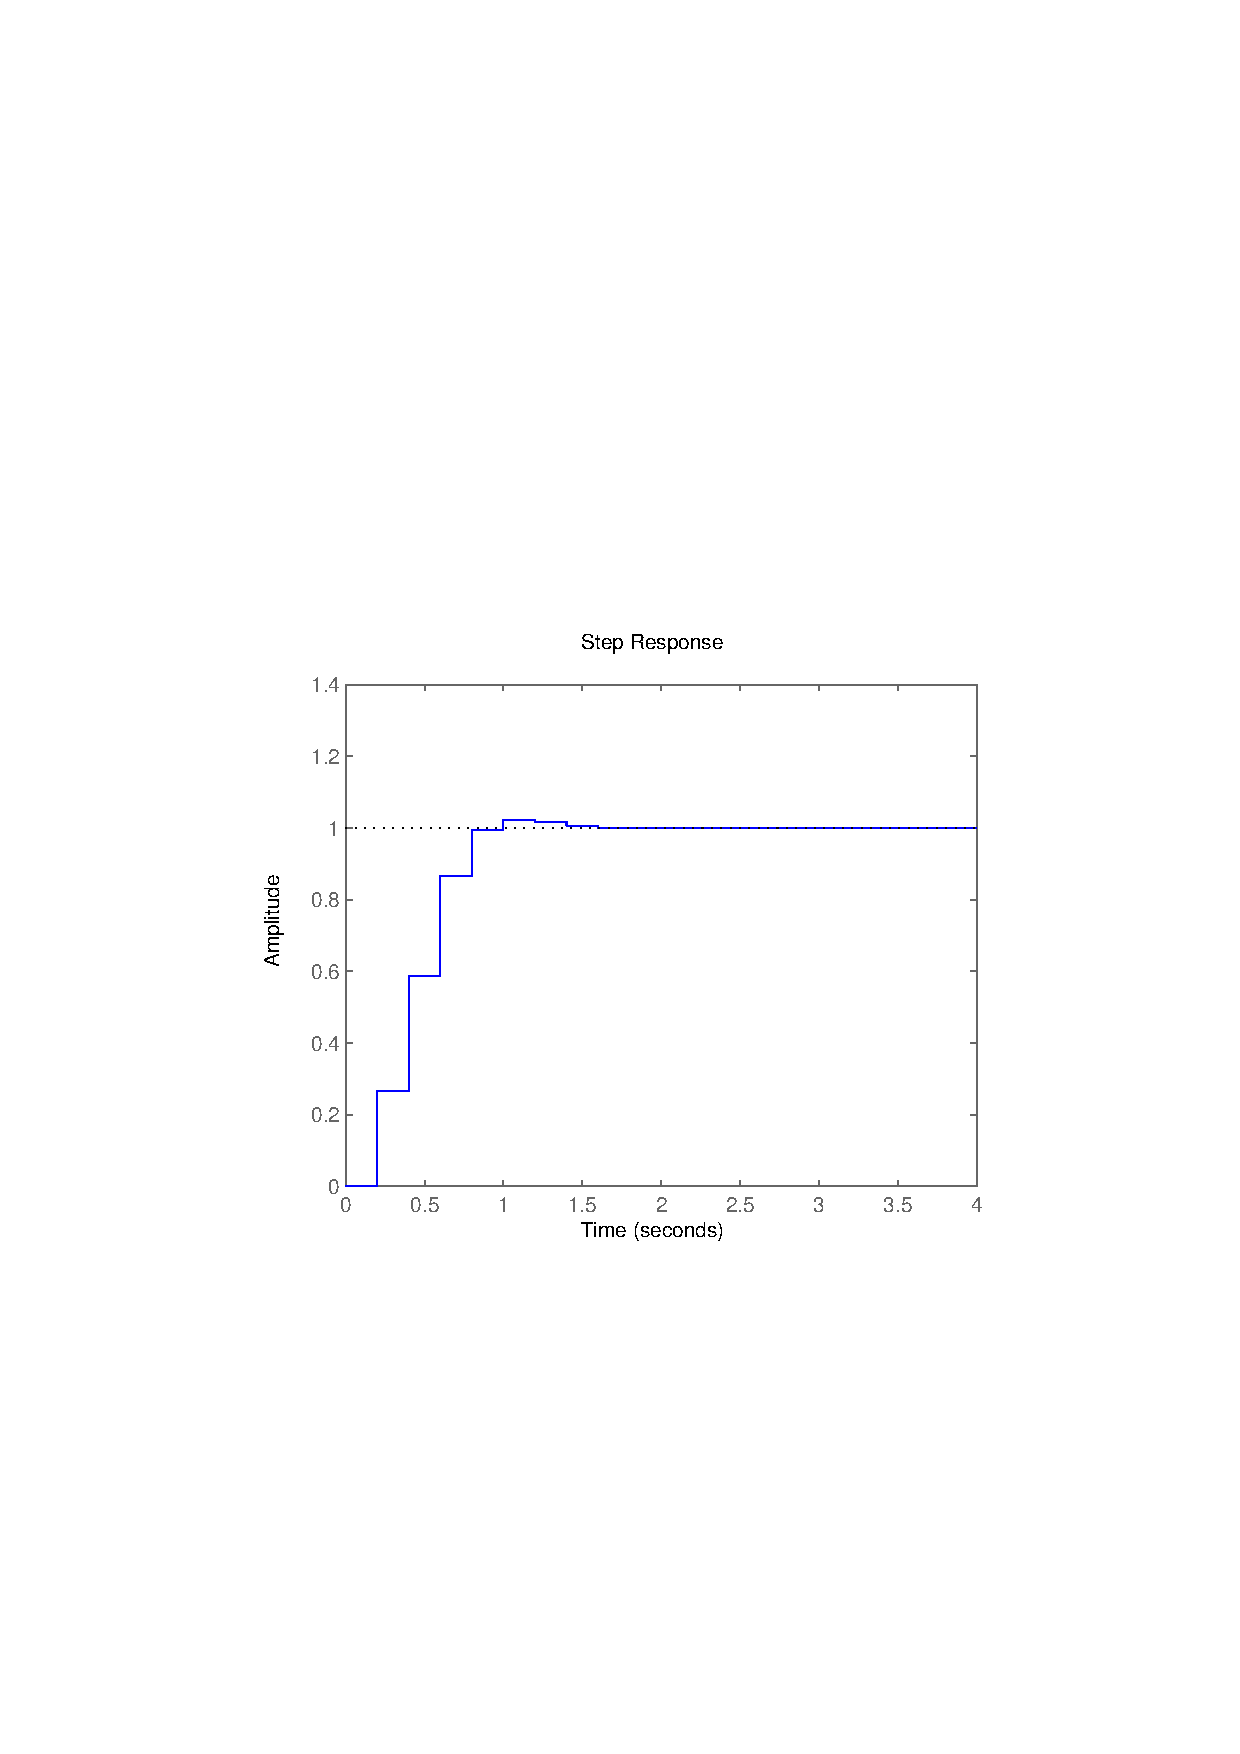
\includegraphics[width=\textwidth]{figures/runningexample_step2.pdf}
        \caption{Final solution by \tool}
        \label{fig:step2}
    \end{subfigure}
\end{figure}
The Original Controller was synthesised ignoring FWL effects and as can be seen, it becomes unstable over time.
\end{frame}
%
\begin{frame}[fragile]{Synthesised Results}
\begin{figure}
 \begin{tikzpicture}
\begin{axis}[ylabel=order,xlabel=time,xmode=log
]
\addplot[scatter,only marks,mark=*] table{./results.dat};
\end{axis}
\end{tikzpicture}
\end{figure}
\end{frame}

\begin{frame}[fragile]{Synthesised Results}

\begin{table}
\centering
\scalebox{0.6}{
\begin{tabular}{| r | c | l | r r || r | r |}
\hline
\# & Plant  & Benchmark                  & $I$ & $F$
   & 2-stage & 1-stage
    \\\hline\hline
1  & $G_{1a}$  & CruiseControl02
            &   4 &  16 & \textbf{12\,s}   & 67\,s     \\
2  & $G_{1b}$  & CruiseControl02$^\dagger$
            &   4 &  16 & 14600\,s   & \textbf{52\,s}     \\
3  & $G_{2a}$  & SpgMsDamper
            &  15 &  16 & \textbf{52\,s}   & 318\,s     \\
4  & $G_{2b}$  & SpgMsDamper$^\dagger$
            &  15 &  16 & \xmark  & \xmark    \\
5  & $G_{3a}$  & SatelliteB2
            &   3 &   7 & \textbf{36\,s}    & \xmark     \\
6  & $G_{3b}$  & SatelliteB2$^\dagger$
            &   3 &   7 & \xmark  & \textbf{4111\,s}  \\
7  & $G_{3c}$  & SatelliteC2
            &   3 &   5 & \textbf{3\,s}    & 205\,s    \\
8  & $G_{3d}$  & SatelliteC2$^\dagger$
            &   3 &   5 & \textbf{50\,s}  & 1315\,s    \\
9  & $G_4$  & Cruise
            &   3 &   7 & 1\,s  & 1\,s    \\
10 & $G_5$  & DCMotor
            &   3 &   7 & \textbf{1\,s}  & 10\,s    \\
11 & $G_6$  & DCServomotor
            &   4 &  11 & \textbf{46\,s}  & \xmark    \\
12 & $G_7$  & Doyleetal
            &   4 &  11 & \textbf{8769\,s}  & \xmark    \\
13 & $G_8$  & Helicopter
            &   3 &   7 & \textbf{44\,s}  & \xmark    \\
14 & $G_9$  & Pendulum
            &   3 &   7 & \textbf{1\,s}  & 14826\,s    \\
15 &$G_{10}$& Suspension
            &   3 &   7 & \textbf{1\,s}  & 5\,s    \\
16 &$G_{11}$& Tapedriver
            &   3 &   7 & 1\,s  & 1\,s    \\
17 &$G_{12a}$& a\_ST1\_IMPL1
            &  16 &   4 & \textbf{11748\,s} & \xmark   \\
18 &$G_{12a}$& a\_ST1\_IMPL2
            &  16 &   8 & \textbf{351\,s}  & \xmark   \\
19 &$G_{12a}$& a\_ST1\_IMPL3
            &  16 &  12 & \textbf{8772\,s}   & \xmark   \\
20 &$G_{12b}$& a\_ST2\_IMPL1
            &  16 &   4 & \textbf{1128\,s}  & \xmark   \\
21 &$G_{12b}$& a\_ST2\_IMPL2
            &  16 &   8 & \xmark  & \xmark    \\
22 &$G_{12b}$& a\_ST2\_IMPL3
            &  16 &  12 & \textbf{15183\,s} & \xmark   \\ 
23 &$G_{12c}$& a\_ST3\_IMPL1
            &  16 &   4 & \xmark & \xmark   \\\hline
\end{tabular}}\\[0.2ex]
\caption{\tool results ({\xmark} = time-out, $\dagger$ = 
uncertainty)
\label{tab:results}}
\end{table}
\end{frame} 

\begin{frame}{Conclusions}
\begin{itemize}
\item We have presented a method for automatically synthesizing stable and sound controllers, implemented
in a tool called \tool.
\item \tool marks the first use of the
CEGIS that handles plants with uncertain models and FWL effects over the
digital controller.  
\item Our experimental results show that \tool is able to synthesize
stable controllers for most benchmarks within a reasonable amount of time.  
\item Future work will extend this CEGIS-based
approach to LTI systems with state space safety specifications. 
\end{itemize}
\end{frame}
\end{document}
